\documentclass[11pt, a4paper]{report}
%\documentclass[11pt, a4paper]{article}

%====================== PACKAGES ======================

\usepackage[french]{babel}
\frenchbsetup{StandardLists=true}
\usepackage{enumitem}
\usepackage{pifont}
\usepackage[utf8x]{inputenc}
%pour gérer les positionnement d'images
\usepackage{float}
\usepackage{amsmath}
\DeclareMathOperator{\dt}{dt}
\usepackage{graphicx}
\usepackage{tabularx}
\usepackage[colorinlistoftodos]{todonotes}
\usepackage{url}
%pour les informations sur un document compilé en PDF et les liens externes / internes
\usepackage[pdfborder=0]{hyperref}
\hypersetup{
	colorlinks = true
	}
%pour la mise en page des tableaux
\usepackage{array}
\usepackage{tabularx}
\usepackage{multirow}
\usepackage{multicol}
\setlength{\columnsep}{50pt}
%pour utiliser \floatbarrier
%\usepackage{placeins}
%\usepackage{floatrow}
%espacement entre les lignes
\usepackage{setspace}
%modifier la mise en page de l'abstract
\usepackage{abstract}
%police et mise en page (marges) du document
\usepackage[T1]{fontenc}
\usepackage[top=2cm, bottom=2cm, left=2cm, right=2cm]{geometry}
%Pour les galerie d'images
\usepackage{subfig}

\usepackage{pdfpages}
\usepackage{tikz}

\usepackage{appendix}

\usepackage{comment}

\usetikzlibrary{angles, quotes}
\usetikzlibrary{decorations.pathmorphing}
%====================== INFORMATION ET REGLES ======================

%rajouter les numérotation pour les \paragraphe et \subparagraphe
\setcounter{secnumdepth}{4}
\setcounter{tocdepth}{4}

\hypersetup{							% Information sur le document
pdfauthor = {Stephan Runigo},			% Auteurs
pdftitle = {Documentation SiCP2},			% Titre du document
pdfsubject = {Documentation du simulateur de chaine de pendules},		% Sujet
pdfkeywords = {SiCP, chaine de pendules},	% Mots-clefs
pdfstartview={FitH}}	% ajuste la page à la largeur de l'écran
%pdfcreator = {MikTeX},% Logiciel qui a crée le document
%pdfproducer = {} % Société avec produit le logiciel
%======================== DEBUT DU DOCUMENT ========================
%
\begin{document}
%
%régler l'espacement entre les lignes
\newcommand{\HRule}{\rule{\linewidth}{0.5mm}}
%
%page de garde	%
\begin{titlepage}
\begin{center}

% Upper part of the page. The '~' is needed because only works if a paragraph has started.
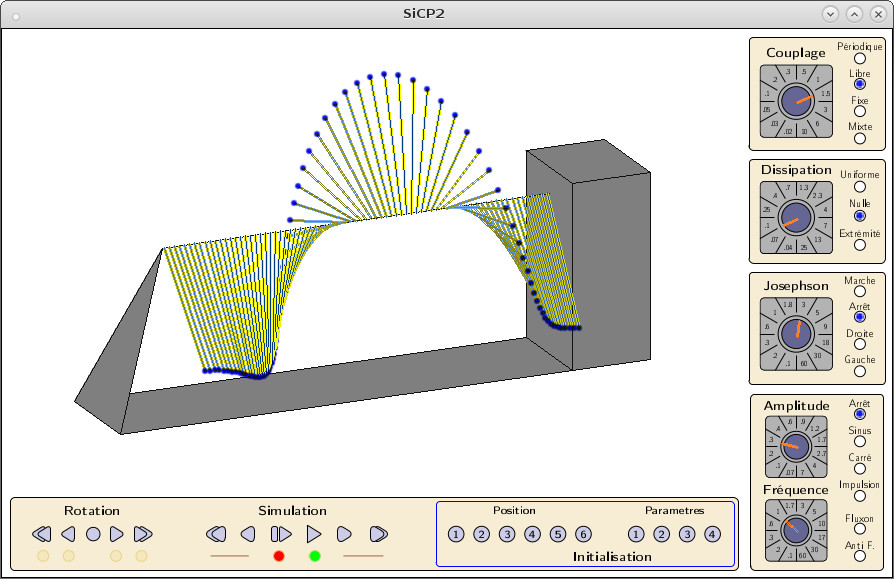
\includegraphics[width=.9\textwidth]{./illustration/SiCP2}
%\caption{SiCF}
\label{fig:image1}
~\\[1cm]


~\\[1cm]

\textsc{\Large }\\[0.5cm]

% Title
\HRule \\[0.4cm]

{\huge \bfseries  SiCP2\\
Documentation et théorie\\[0.4cm] }

\HRule \\[1.5cm]

% Author and supervisor
\begin{minipage}{0.4\textwidth}
\begin{flushleft} \large
%\emph{Auteur:}\\
%Stephan \textsc{Runigo}
\end{flushleft}
\end{minipage}
\begin{minipage}{0.4\textwidth}
\begin{flushright} \large
\emph{Auteur:}\\
Stephan \textsc{Runigo}
\end{flushright}
\end{minipage}

\vfill

% Bottom of the page
{\large \today}

\end{center}
\end{titlepage}

%
%page blanche	%
\begin{center}
\Large
Résumé
\normalsize
\end{center}
\vspace{3cm}
\begin{itemize}[leftmargin=1cm, label=\ding{32}, itemsep=21pt]
\item {\bf Objet : }Ce document accompagne le programme SiCP2.
\item {\bf Contenu : }Il contient un manuel d'installation et d'utilisation ainsi qu'un certain nombre de développements théoriques.
\item {\bf Public concerné : }Les enseignants, les étudiants et les passionnés de physique et d'informatique.
\end{itemize}

\vspace{3cm}

SiCP2 est un simulateur numérique d'équations physiques offrant une représentation graphique et une interaction dynamique avec les paramètres physiques. Destinés à un usage ludique et pédagogique, il permet de visualiser le comportement des systèmes physiques simulés. Cette documentation accompagne ce programme.

\begin{itemize}[leftmargin=1cm, label=\ding{32}, itemsep=11pt]
\item Les deux premiers chapitres présentent SiCP2, présente les procédures d'installation et précisent les commandes permettant l'interaction avec le programme.
\item Les deux chapitres suivants fournissent un certain nombre de développements théoriques liés au phénomènes physiques et à la numérisation des équations.
\item Enfin, le dernier chapitre rassemble les informations liées à la structure du code source.
\end{itemize}

%\newpage
%~
%ne pas numéroter cette page
%\thispagestyle{empty}
	%\newpage

\tableofcontents
\thispagestyle{empty}
\setcounter{page}{0}
%ne pas numéroter le sommaire
%
%\newpage
%
%espacement entre les lignes d'un tableau
\renewcommand{\arraystretch}{1.5}
%
%====================== INCLUSION DES PARTIES ======================
%
~
\thispagestyle{empty}
%recommencer la numérotation des pages à "1"
\setcounter{page}{0}
\newpage
%	%
%
%

%%%%%%%%%%%%%%%%%%%%%%%%%%%%%%%%%%
\chapter{Présentation}
%%%%%%%%%%%%%%%%%%%%%%%%%%%%%%%%%%

%
\section{SiCP2, chaîne de pendules couplés}
%
SiCP2 est un simulateur de chaîne de pendule. Un moteur sinusoïdale, carré, ou impulsionnel permet de créer une excitation de l'extrémité de la chaîne. Les conditions aux limites peuvent être périodiques, libres ou fixes. La dissipation peut être uniforme ou simuler une extrémité absorbante.
%
\begin{center}
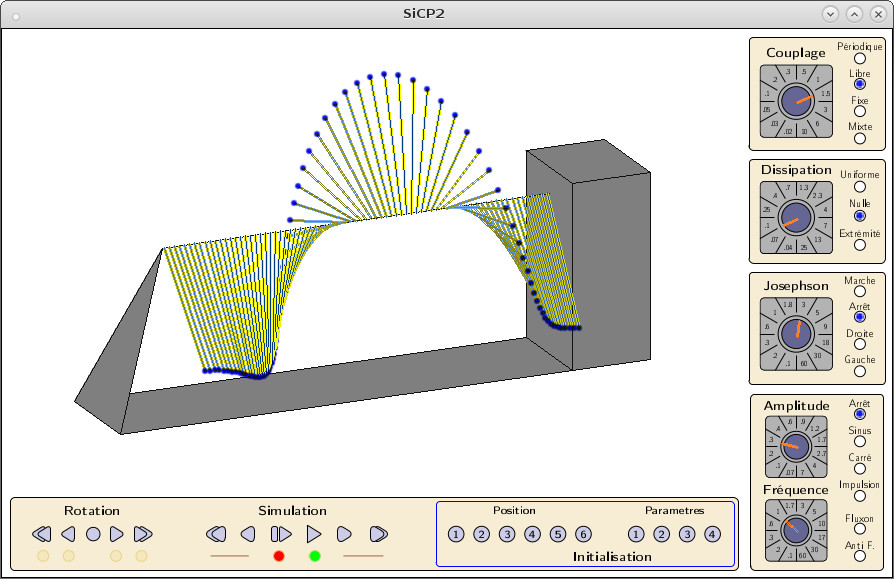
\includegraphics[scale=0.41]{./illustration/SiCP2}
\end{center}
%
Le programme simule l'équation de sine-gordon. Le contrôle du courant josephson permet d'observer la dynamique des solitons.
%
%%%%%%%%%%%%%%%%%%%%%%%%%%%%%%%%%%%%%%%%%%%%%%%%%%%%%%%%%%%%%%%%%%%%%%%%%%%%%%%%%%%%%%%%%%%%%

%
\section{Installation de SiCP2}
%
\subsection{Exécutable pour Windows}
%
\begin{center}
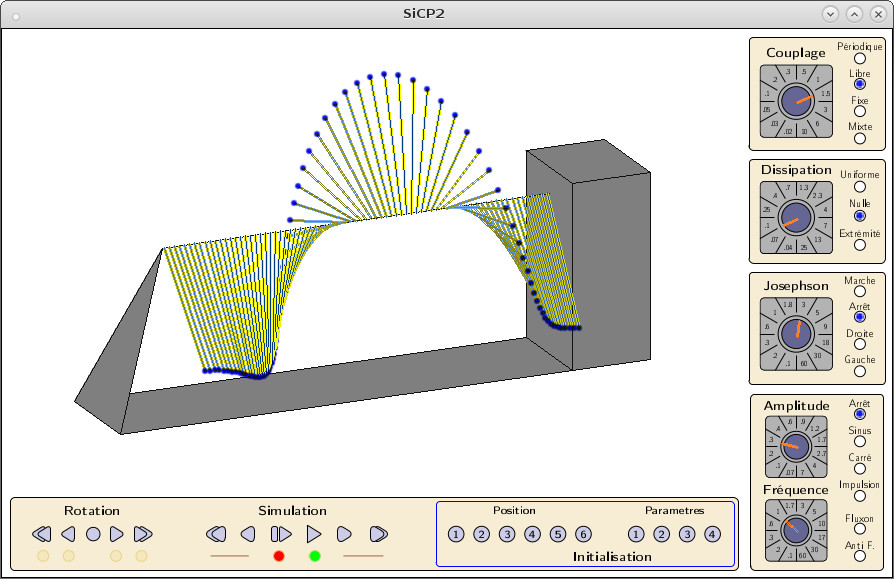
\includegraphics[width=.9\textwidth]{./illustration/SiCP2}
\end{center}
%
https://github.com/Cphysique/SiCP2/
https://cphysique.github.io/
%
\subsection{Compilation du code source}
%
Le bouton vert de la page 
%
\begin{center}
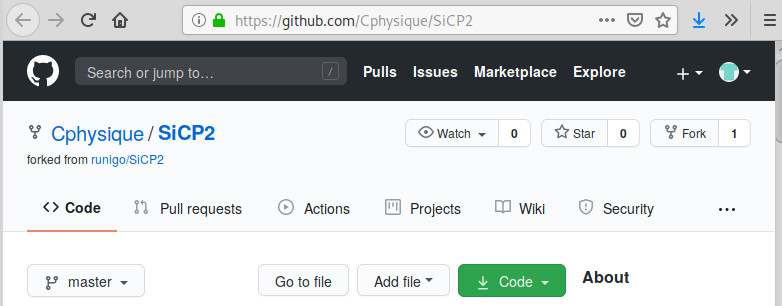
\includegraphics[width=.9\textwidth]{./presentation/CphysiqueSiCP2}
\end{center}
%
%
\begin{center}
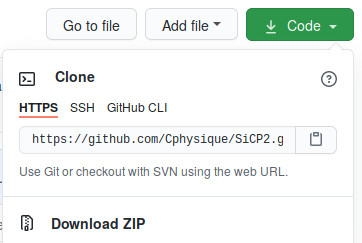
\includegraphics[width=.9\textwidth]{./presentation/CphysiqueSiCP2code}
\end{center}
%
Cette section traite de l'installation des simulateurs SiTS2, SiCF2 et SiCP2 sur un système d'exploitation de type debian. Le téléchargement se fait avec un navigateur internet, la compilation et l'exécution se font dans un terminal. L'installation des outils de compilation nécessite les privilèges du super-utilisateur.
\begin{itemize}[leftmargin=1cm, label=\ding{32}, itemsep=0pt]
\item {\bf Installation des outils de compilation}
Avec les droits du super-utilisateur
	\begin{itemize}[leftmargin=1cm, label=\ding{32}, itemsep=0pt]
	\item \texttt{apt-get install gcc make libsdl-dev}
	\item Pour les versions 2 des simulateurs, installer la librairie SDL2 :
	\item \texttt{apt-get install libsdl2-dev}
	\end{itemize}
\item {\bf Téléchargement des sources}
	\begin{itemize}[leftmargin=1cm, label=\ding{32}, itemsep=0pt]
	\item Télécharger les fichiers \texttt{.zip} sur github
		\begin{itemize}[leftmargin=1cm, label=\ding{32}, itemsep=0pt]
		\item \texttt{https://github.com/runigo/SiCP2/archive/master.zip}
		\item \texttt{https://github.com/runigo/SiCF2/archive/master.zip}
		\item \texttt{https://github.com/runigo/SiTS2/archive/master.zip}
		\end{itemize}
	\item Décompresser les fichiers \texttt{.zip}
		\begin{itemize}[leftmargin=1cm, label=\ding{32}, itemsep=0pt]
		\item \texttt{unzip SiCP2-master.zip}
		\item \texttt{unzip SiCF2-master.zip}
		\item \texttt{unzip SiTS2-master.zip}
		\end{itemize}
	\end{itemize}
\item {\bf Compilation}
	\begin{itemize}[leftmargin=1cm, label=\ding{32}, itemsep=0pt]
	\item La commande \texttt{make} dans le répertoire des sources produit un fichier exécutable :
		\begin{itemize}[leftmargin=1cm, label=\ding{32}, itemsep=0pt]
		\item \texttt{SiCP2} pour SiCP
		\item \texttt{SiCF2} pour SiCF
		\item \texttt{SiTS2} pour SiTS
		\end{itemize}
	\end{itemize}
%
\item {\bf Exécution}
	\begin{itemize}[leftmargin=1cm, label=\ding{32}, itemsep=0pt]
	\item En ligne de commande, avec d'éventuelles options
		\begin{itemize}[leftmargin=1cm, label=\ding{32}, itemsep=0pt]
		\item \texttt{./SiCP2 [OPTION]}
		\item \texttt{./SiCF2 [OPTION]}
		\item \texttt{./SiTS2 [OPTION]}
		\end{itemize}
	\item La fenêtre graphique donne une représentation de la simulation,
	\item Le terminal affiche les informations.
	\end{itemize}
\end{itemize}

%%%%%%%%%%%%%%%%%%%%%%%%%%%%%%%%%%%%%%%%%%%%%%%%%%%%%%%%%%%%%%%%%%%%%%%%%%%%%%%%%%%%%%%%%%%%%

%
%%%%%%%%%%%%%%%%%%%%%%
\section{Exemples}
%%%%%%%%%%%%%%%%%%%%%%

Cette section traite de la mise en marche et des premières utilisation de SiCF

\subsection{Dissipation}
\begin{itemize}[label=\ding{32}, leftmargin=2cm]
\item \texttt{texte} : texte
\end{itemize}
%
\subsection{Conditions aux limites}
\begin{itemize}[label=\ding{32}, leftmargin=2cm]
\item Périodique
\item libre
\item fixe
\end{itemize}
%
\subsection{Transformée de fourier}
%
\subsection{Réalisation d'un paquet d'onde}
%
\subsection{Inégalité de Heisenberg}
%
\subsection{}



%%%%%%%%%%%%%%%%%%%%%%%%%%%%%%%%%%%%%%%%%%%%%%%%%%%%%%%%%%%%%%%%%%%%%%


%
%
%
\section{Installation de SiCP2}
%
\subsection{Exécutable pour Windows}
%
\begin{center}
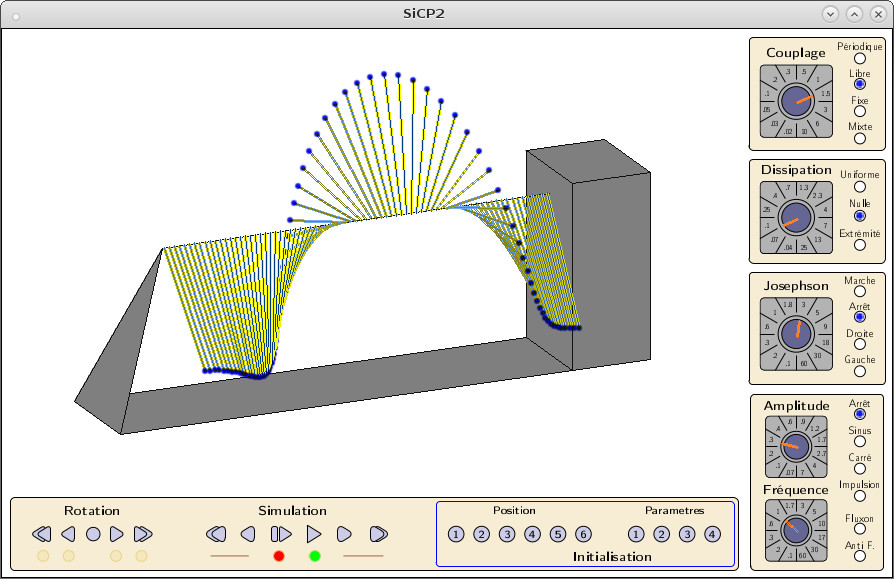
\includegraphics[width=.9\textwidth]{./illustration/SiCP2}
\end{center}
%
https://github.com/Cphysique/SiCP2/
https://cphysique.github.io/
%
\subsection{Compilation du code source}
%
Le bouton vert de la page 
%
\begin{center}
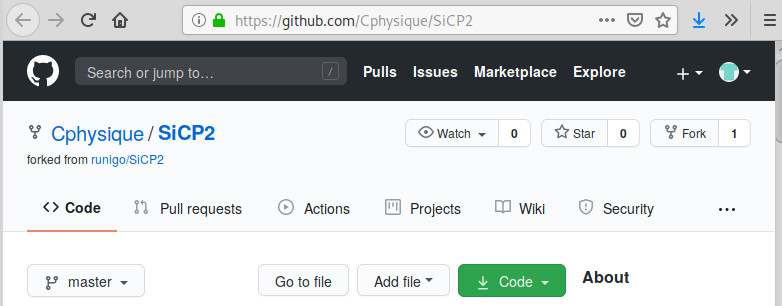
\includegraphics[width=.9\textwidth]{./presentation/CphysiqueSiCP2}
\end{center}
%
%
\begin{center}
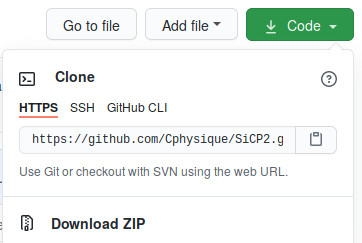
\includegraphics[width=.9\textwidth]{./presentation/CphysiqueSiCP2code}
\end{center}
%
Cette section traite de l'installation des simulateurs SiTS2, SiCF2 et SiCP2 sur un système d'exploitation de type debian. Le téléchargement se fait avec un navigateur internet, la compilation et l'exécution se font dans un terminal. L'installation des outils de compilation nécessite les privilèges du super-utilisateur.
\begin{itemize}[leftmargin=1cm, label=\ding{32}, itemsep=0pt]
\item {\bf Installation des outils de compilation}
Avec les droits du super-utilisateur
	\begin{itemize}[leftmargin=1cm, label=\ding{32}, itemsep=0pt]
	\item \texttt{apt-get install gcc make libsdl-dev}
	\item Pour les versions 2 des simulateurs, installer la librairie SDL2 :
	\item \texttt{apt-get install libsdl2-dev}
	\end{itemize}
\item {\bf Téléchargement des sources}
	\begin{itemize}[leftmargin=1cm, label=\ding{32}, itemsep=0pt]
	\item Télécharger les fichiers \texttt{.zip} sur github
		\begin{itemize}[leftmargin=1cm, label=\ding{32}, itemsep=0pt]
		\item \texttt{https://github.com/runigo/SiCP2/archive/master.zip}
		\item \texttt{https://github.com/runigo/SiCF2/archive/master.zip}
		\item \texttt{https://github.com/runigo/SiTS2/archive/master.zip}
		\end{itemize}
	\item Décompresser les fichiers \texttt{.zip}
		\begin{itemize}[leftmargin=1cm, label=\ding{32}, itemsep=0pt]
		\item \texttt{unzip SiCP2-master.zip}
		\item \texttt{unzip SiCF2-master.zip}
		\item \texttt{unzip SiTS2-master.zip}
		\end{itemize}
	\end{itemize}
\item {\bf Compilation}
	\begin{itemize}[leftmargin=1cm, label=\ding{32}, itemsep=0pt]
	\item La commande \texttt{make} dans le répertoire des sources produit un fichier exécutable :
		\begin{itemize}[leftmargin=1cm, label=\ding{32}, itemsep=0pt]
		\item \texttt{SiCP2} pour SiCP
		\item \texttt{SiCF2} pour SiCF
		\item \texttt{SiTS2} pour SiTS
		\end{itemize}
	\end{itemize}
%
\item {\bf Exécution}
	\begin{itemize}[leftmargin=1cm, label=\ding{32}, itemsep=0pt]
	\item En ligne de commande, avec d'éventuelles options
		\begin{itemize}[leftmargin=1cm, label=\ding{32}, itemsep=0pt]
		\item \texttt{./SiCP2 [OPTION]}
		\item \texttt{./SiCF2 [OPTION]}
		\item \texttt{./SiTS2 [OPTION]}
		\end{itemize}
	\item La fenêtre graphique donne une représentation de la simulation,
	\item Le terminal affiche les informations.
	\end{itemize}
\end{itemize}

%%%%%%%%%%%%%%%%%%%%%%%%%%%%%%%%%%%%%%%%%%%%%%%%%%%%%%%%%%%%%%%%%%%%%%%%%%%%%%%%%%%%%%%%%%%%%

\newpage
\chapter{Utilisation des simulateurs}
%%%%%%%%%%%%%%%%%%%%%%%%%%%%%%%%%%%%%
%\section{Utilisation des simulateurs}
%%%%%%%%%%%%%%%%%%%%%%%%%%%%%%%%%%%%%

Ce chapitre traite des interactions entre le programme et l'utilisateur.

%%%%%%%%%%%%%%%%%%%%%%%%%%%%%%%%%%%%%%%%%%%%%%%%%%%%%%%%%%
%
\section{Commandes communes avec SiCF}
%
%%%%%%%%%%%%%%%%%%%%%%%%%%%%%%%%%%%%%%%%%%%%%%%%%%%%%%%%%%
%
%
\subsection{Options de la ligne de commande}
%
Lorsque le programme est démarré en ligne de commande, il est possible de passer un certain nombre d'options. Ces options sont communiquées au programme à l'aide du nom de l'option suivie d'un nombre. Par exemple pour démarrer SiCP2 avec un nombre de pendules égale à 50 :
\begin{center}
\texttt{./SiCP2 nombre 50}
\end{center}
%
Pour démarrer SiCP2 en exploitant plusieurs options :
\begin{center}
\texttt{./SiCP2 support 0 pause 7 duree 998 dt 0.0027 nombre 777}
\end{center}
%
\subsubsection{Résumé des options}
\begin{center}
\begin{tabular}{cccc}
option & valeur & clavier & commande \\
%\hline
{\texttt dt} & (dt > 0.0 \& dt < DT\_MAX) &  & discrétisation du temps \\
{\texttt duree} & () & {\sf F9}, {\sf F10}, {\sf F11}, {\sf F12} & rythme de la simulation \\
{\texttt mode} & () & {\sf Entrée} & Mode -1 : Wait, 1 : Poll \\
{\texttt nombre} & (nombre > 0 \& nombre < 1099) &  & Nombre de pendules\\
{\texttt aide} & () &  & Affiche l'aide \\
{\texttt help} & () &  & Affiche l'aide \\
\end{tabular}
\end{center}

{\it
* Initialise le déphasage entre le dernier pendule et le premier pendule dans le cas des conditions aux limites périodique.

}
%
%
\subsection{Commades du clavier}
%
%
\subsubsection{Variations des paramètres}
%
%
\subsubsection{Enregistrement et réinitialisation des situations}
%

Lorsque la touche {\sf Maj} est enfoncée, l'appui sur une touche alphabétique ré-initialise le système dans la configuration correspondant à la touche.

Lorsque les touches {\sf Ctrl} et {\sf Maj} sont enfoncées, l'appui sur une touche alphabétique enregistre la configuration présente du système à la place de la configuration correspondant à la touche. La nouvelle configuration enregistrée peut alors ré-initialiser le système grâce à la touche {\sf Maj}

Lorsque la touche {\sf Ctrl} est enfoncée, l'appui sur une touche alphabétique ré-initialise le système dans la configuration d'origine de SiCP2 correspondant à la touche.

%Les fichiers de ré-initialisation se trouvent dans le répertoire {\texttt donnee/enregistrement}. Ils peuvent être édités. Le nom de ces fichiers doit être respecté afin de pouvoir être ouvert par le programme (ces noms sont utilisés par {\texttt donnees/fichier.c}).
%

%%%%%%%%%%%%%%%%%%%%%%%%%%%%%%%%%%%%%%%%%%%%%%%%%%%%%%%%%%
%
\section{SiCP2}
%
%%%%%%%%%%%%%%%%%%%%%%%%%%%%%%%%%%%%%%%%%%%%%%%%%%%%%%%%%%
%
SiCP2 possède une interface graphique permettant de modifier les paramètres à l'aide de la souris.
%
\subsection{Panneau de droite}
%
Ce panneau possède cinq boutons rotatifs et 17 boutons "radio". La rotation s'effectue en plaçant le pointeur de la souris sur l'un des boutons rotatif et en actionnant la molette. La sélection d'un bouton radio s'effectue en cliquant sur celui-ci. 
%
%
\begin{itemize}[leftmargin=1cm, label=\ding{32}, itemsep=0pt]
	\item {\bf Couplage} : change le couplage élastique entre les pendules
	\begin{itemize}[leftmargin=1cm, label=\ding{32}, itemsep=0pt]
		\item Périodique : couple le premier pendule au dernier
		\item Libre : libère le premier et le dernier pendule
		\item Fixe : fixe le premier et le dernier pendule
		\item Mixte : fixe le premier et libère le dernier pendule
	\end{itemize}
	\item {\bf Dissipation} : change le frotement visqueux sur les pendules
	\begin{itemize}[leftmargin=1cm, label=\ding{32}, itemsep=0pt]
		\item Uniforme : installe un frottement visqueux uniforme
		\item Nulle : anulle le frottement visqueux
		\item Extrémité : installe un frottement visqueux croissant sur les derniers pendules (1/6 de la chaîne)
	\end{itemize}
	\item {\bf Josephson} : change l'amplitude du courant josephson
	\begin{itemize}[leftmargin=1cm, label=\ding{32}, itemsep=0pt]
		\item Marche : démarre le courant josephson
		\item Arrêt : arrête le courant josephson
		\item Droite / Gauche : change le sens du courant josephson
	\end{itemize}
	\item {\bf Amplitude} : change l'amplitude du moteur périodique
	\item {\bf Fréquence} : change la fréquence du moteur périodique
	\begin{itemize}[leftmargin=1cm, label=\ding{32}, itemsep=0pt]
		\item Arrêt : arrête le moteur périodique
		\item Sinus : démarre le moteur sinusoïdale
		\item Carré : démarre le moteur carré
		\item Impulsion : démarre le moteur sinusoïdale et l'arrête après une période
	\end{itemize}
	\begin{itemize}[leftmargin=1cm, label=\ding{32}, itemsep=0pt]
		\item FLuxon : ajoute un déphasage de 2$\pi$ au premier pendule. Le fluxon n'apparaît pas si les extrémités sont libres.
		\item Anti. F : retranche un déphasage de 2$\pi$ au premier pendule
	\end{itemize}
\end{itemize}
%
%
\subsection{Panneau du bas}
%
La sélection d'un bouton radio s'effectue en cliquant sur celui-ci. 
%
%
\begin{itemize}[leftmargin=1cm, label=\ding{32}, itemsep=0pt]
	\item Rotation : démarre la rotation du point de vue
	\begin{itemize}[leftmargin=1cm, label=\ding{32}, itemsep=0pt]
		\item rotation vers la droite
		\item arrête la rotation
		\item rotation vers la gauche
	\end{itemize}
	\item Simulation : contrôle la rapidité de la simulation
	\begin{itemize}[leftmargin=1cm, label=\ding{32}, itemsep=0pt]
		\item ralentie la simulation
		\item arrête / démarre la simulation
		\item temps réel
		\item accélère la simulation
	\end{itemize}
	\item Initialisation : Réinitialise le système
	\begin{itemize}[leftmargin=1cm, label=\ding{32}, itemsep=0pt]
		\item réinitialisation de la position des pendules
		\item réinitialisation des paramètres et du nombre de pendules
	\end{itemize}
\end{itemize}
%
\subsection{Panneau central}
%
Le panneau centrale montre la chaîne de pendule. Le point de vue se déplace en maintenant le clic de la souris et en déplaçant celle-ci. La molette permet de changer la distance du point de vue.
%
%
%%%%%%%%%%%%%%%%%%%%%%%%%%%%%%%%%%%%%%%%%%%%%%%%%%%%%%%%%



%
%
%%%%%%%%%%%%%%%%%%%%%%
\section{Exemples}
%%%%%%%%%%%%%%%%%%%%%%

Cette section traite de la mise en marche et des premières utilisation de SiCF

\subsection{Dissipation}
\begin{itemize}[label=\ding{32}, leftmargin=2cm]
\item \texttt{texte} : texte
\end{itemize}
%
\subsection{Conditions aux limites}
\begin{itemize}[label=\ding{32}, leftmargin=2cm]
\item Périodique
\item libre
\item fixe
\end{itemize}
%
\subsection{Transformée de fourier}
%
\subsection{Réalisation d'un paquet d'onde}
%
\subsection{Inégalité de Heisenberg}
%
\subsection{}



%%%%%%%%%%%%%%%%%%%%%%%%%%%%%%%%%%%%%%%%%%%%%%%%%%%%%%%%%%%%%%%%%%%%%%


%
\chapter{Modèle physique}
%
Ce chapitre traite du modèle physique de la chaîne de pendules.
%
%%%%%%%%%%%%%%%%%%%%%%%%%%%%%%
\section{La chaîne de pendule}
%%%%%%%%%%%%%%%%%%%%%%%%%%%%%%

\label{polytechnique-sujet}
\label{polytechnique-corrige}

Sujet polytechnique \cite{soliton-sujet} \cite{soliton-corrige}
\subsection{Le pendule pesant}
\begin{multicols}{2}%\columnbreak\end{multicols}
\begin{tikzpicture}
%\draw [ball color=gray] (0,0)coordinate(A)node[left]{$m$\ \ \ } circle (.3);
\draw [ball color=gray] (0,0)coordinate(A)node[below=3mm]{$m$} circle (.3);
\draw (0.21,0.21) -- (45:4.7)coordinate(B)node[right]{O}node[pos=.5,left=2mm]{$l$};
%\draw (0,0)coordinate(A)node[left]{m}circle(.1)-- (40:5)coordinate(B)node[right]{O};=3mm
\draw[dashed](B)--++(0,-5)coordinate(C);
\draw pic[ draw ,<->,"$\theta$",angle eccentricity =1.5, angle radius=1cm]{ angle =A--B--C};
%\draw[dotted,thick](0,0)arc(-135:-90:5);node[right]{B}
\draw [->](5,2) --++(0,-2)node[pos=.5,left]{$\overrightarrow{g}$};
\end{tikzpicture}

\columnbreak
Un pendule pesant est constitué par une masse $m$ suspendue à un fil rigide de longueur $l$ relié à un point O. Une liaison en ce point permet au pendule de tourner autour d'un axe fixe. L'angle entre le fil et la verticale est noté $\theta$. La masse est soumise à son poids $\overrightarrow{P}=m\overrightarrow{g}$, à la réaction du fil $\overrightarrow{R}$ et à une force de frottement visqueux $\overrightarrow{f}= - \frac{\beta}{l} \overrightarrow{v}$. La relation fondamentale de la dynamique donne :
\[
m l\ \frac{d^2 \theta}{\dt^2} =  - m g \sin{\theta}  -  \beta\ \frac{d \theta}{\dt}
\]
\end{multicols}
%
\subsection{Les pendules couplés}
\begin{multicols}{2}%\columnbreak\end{multicols}
Deux pendules pesants sont reliés par un fil de torsion suivant leur axe fixe commun.  La relation fondamentale de la dynamique donne alors :
\[\left\{
  \begin{array}{rcr}
m l\ \frac{d^2 \theta _1}{\dt^2} & = &  - m g \sin{\theta _1}  -  \beta\ \frac{d \theta _1}{\dt} - kl (\theta _1 - \theta _2) \\
m l\ \frac{d^2 \theta _2}{\dt^2} & = &  - m g \sin{\theta _2}  -  \beta\ \frac{d \theta _2}{\dt} - kl (\theta _2 - \theta _1) \\
  \end{array}
\right.\]
dans le cas où les pendules sont identiques.

\columnbreak
\begin{tikzpicture}
\draw [ball color=gray] (0,0)coordinate(A)node[below=3mm]{$m$} circle (.2);
\draw (0.13,0.13) -- (65:2.7)coordinate(B);%node[right]{O}node[pos=.5,left=2mm]{$l$};
\draw[dashed](B)--++(0,-3)coordinate(C);
\draw pic[ draw ,<->,"$\theta _1$",angle eccentricity =1.5, angle radius=1cm]{ angle =A--B--C};
%
\draw [ball color=gray] (3,0.3)coordinate(D)node[below=3mm]{$m$} circle (.2);
\draw (3.13,0.43) -- (35:5.1)coordinate(E);%node[right]{O}node[pos=.5,left=2mm]{$l$};
\draw[dashed](E)--++(0,-3)coordinate(F);
\draw pic[ draw ,<->,"$\theta _2$",angle eccentricity =1.5, angle radius=1cm]{ angle =D--E--F};
%
\draw[decorate,decoration={coil,segment length=10pt,amplitude=0.2cm,aspect=.8}](B)--(E)node[pos=.5,above=2mm]{$k$};
\end{tikzpicture}
\end{multicols}
%
%
%
\subsection{La chaîne de pendule}
Une chaîne de pendule est constituée d'une série de pendules pesants. Chaque pendule étant couplé avec ses deux plus proches voisins à l'aide d'un fil de torsion.

\begin{tikzpicture}[rotate=-10]
\foreach \x/\t/\a in {1/{}/0, 2/{}/2, 3/{}/5, 4/{\theta _{n-1}}/9, 5/{\theta _n}/14, 6/{\theta _{n+1}}/9, 7/{}/5, 8/{}/2, 9/{}/0}
{
\coordinate (A) at (1.5*\x,0) ;
\draw[decorate,decoration={coil,amplitude=0.07cm,aspect=1.1}](A)-- ++(1.5,0)coordinate(B);
\draw (B) -- ++(-90-\a:3)[ball color=gray] ++(0,0) circle (.2) node[below=2mm]{$\t$};
%\draw;
}
\end{tikzpicture}

\subsection{L'équation de la chaine de pendule}
\label{barreteau}
La chaîne de pendule est constituée d'une série de pendules pesants. Chaque pendule étant couplé avec ses deux plus proches voisins à l'aide d'un fil de torsion.\cite{chaine-pendule}
\[
\frac{\mathrm d^2\theta _n}{\mathrm d t^2} - c^2 \frac{\theta _{n+1} + \theta _{n-1} - 2 \theta _n}{\mathrm{a} ^2} + \omega _0 ^2 \sin \theta _n = 0
\]
%
\begin{center}
\begin{tabular}{cccc}
%\multicolumn{4}{|c|}{Contrôles} & \multicolumn{4}{c}{Information} & \multicolumn{4}{|c|}{Contrôles}\\
$\frac{k}{m}$ & $\frac{vitesse^2}{longueur^2}$ & T$^{-2}$ & $\frac{k}{m}$ = $\frac{c^2}{a^2}$ \\
$\frac{g}{l}$& pulsation$^2$ & T$^{-2}$ & $\frac{g}{l}$ = $\omega _0 ^2$ \\
\end{tabular}
\end{center}

La relation fondamentale de la dynamique, donne, en prennant en compte les frottements visqueux :
\[
m l\ \frac{d^2 \theta _n}{\dt^2} =  - m g \sin{\theta _n}  -  k l \Delta \theta _n(t)  -  \beta\ \frac{d \theta _n}{\dt}
\]
soit
\[
\frac{d^2 \theta _n}{\dt^2} =  - \frac{g}{l} \sin{\theta _n}  -  \frac{k}{m} \Delta \theta _n(t)  - \frac{\beta}{ml}\ \frac{d \theta _n}{\dt}
\]
avec
\begin{center}
\begin{tabular}{cccccc}
 & {\it abréviation} & {\it grandeur} & {\it dimension} &  \\
 & $\theta _n$ & angle & radian &  \\
 & m & masse & M &  \\
 & g & pesanteur & LT$^{-2}$ &  \\
 & k & raideur & MT$^{-2}$ &  \\
 & l & longueur & L &  \\
 & $\beta$ & frottement & ML$^{2}$T$^{-1}$ &  \\
\end{tabular}
\end{center}
%
\subsection{Expressions des forces et des énergies associées}

La force de rappel, s'exerçant sur la masse m, dû au fil de torsion ( $C=kl^2$ ) entre les pendules est :
\[
f_{torsion} = -  k l \Delta \theta _n = -  k l\ (2\theta _n-\theta _{n-1}-\theta _{n+1})
\]
L'énergie potentielle entre les pendules n et n-1 est :
\[
E_{couplage} = \frac{1}{2}\ k l^2 (\theta _n-\theta _{n-1})^2
\]

La force de rappel dû à la gravitation est :
\[
f_{gravitation} = - m g \sin{\theta _n}
\]
L'énergie potentielle de pesanteur de la masse m est :
\[
E_{pp} = m g l (1 - \cos{\theta _n})
\]
La linéarisation de cette dernière force donne lieu à une force de rappel harmonique :
\[
f_{ressort} = - m g \theta _n
\]
L'énergie potentielle correspondante est alors:
\[
E_{pp} = \frac{1}{2}\ m g l \theta _n^2
\]

Enfin, l'énergie cinétique découle du travail de 
\[
m l\ \frac{d^2 \theta _n}{\dt^2}
\]
%
Et vaut
\[
E_{c} = \frac{1}{2}\ m l (\frac{d \theta _n}{\dt})^2
\]


La force de frottement visqueux est :
%
\[
f_{frottement} = -  \beta\ \frac{\theta _n(t) - \theta _n(t-\dt)}{\dt}
\]
%
La présence de cette force implique une dissipation de l'énergie. En l'absence de cette force, on doit observer une conservation de l'énergie totale.

À ces forces il faut ajouter le courant josephson, correspondant à une constante additive dans la relation fondamentale de la dynamique ainsi que la force s'exerçant sur le premier pendule lors de l'excitation de la chaîne.
%%%%%%%%%%%%%%%%%%%%%%%%%%%%%%%%%%%%%%%%%%%%%%%%%%%%%%%%%%%%%%%%%
%La relation fondamentale de la dynamique donne :
%\[- m g \sin{\theta _n(t)}  -  k l \Delta \theta _n(t)  -  \beta\ \frac{\theta _n(t) - \theta _n(t-\dt)}{\dt} =  m l\ \frac{\theta _n(t+\dt) - 2\theta _n(t) + \theta _n(t-\dt)}{\dt^2}\]
%soit\[\frac{\theta _n(t+\dt) - 2\theta _n(t) + \theta _n(t-\dt)}{\dt^2} = - \frac{g}{l} \sin{\theta _n(t)}  -  \frac{k}{m} \Delta \theta _n(t)  -  \frac{\beta}{ml}\ \frac{\theta _n(t) - \theta _n(t-\dt)}{\dt}\]
%D'ou finallement\[\theta _n(t+\dt) = 2\theta _n(t) - \theta _n(t-\dt) + \delta force_n\]
%avec \[\delta force_n = - \dt^2 \frac{g}{l} \sin{\theta _n(t)} - \dt^2 \frac{k}{m} \Delta \theta _n(t) - \dt \frac{\beta}{ml} (\theta _n(t) - \theta _n(t-\dt))\]
%%%%%%%%%%%%%%%%%%%%%%%%%%%%%%%%%%%%%%%%%%%%%%%%%%%%%%%%%%%%%%%%%
\subsection{Résumé des forces et des énergies}
\begin{center}
\begin{tabular}{ccc}
%\multicolumn{4}{|c|}{Contrôles} & \multicolumn{4}{c}{Information} & \multicolumn{4}{|c|}{Contrôles}\\
 & force & énergie \\
torsion & -  k l $\Delta \theta _n$ & $\frac{1}{2}$ k l$^2 (\theta _n-\theta _{n-1})^2$ \\
gravitation & - m g $\sin{\theta _n}$ & m g l (1 - $\cos{\theta _n}$) \\
harmonique & - m g $\theta _n$ & $\frac{1}{2}$ m g l $\theta _n^2$ \\
inertie & m l $\frac{d^2 \theta _n}{\dt^2}$ & $\frac{1}{2}$ m l$^2$ $(\frac{d \theta _n}{\dt})^2$ \\
courant & josephson & \\
\end{tabular}
\end{center}
%

%
%%%%%%%%%%%%%%%%%%%%%
\section{L'équation de Sine-Gordon}
%%%%%%%%%%%%%%%%%%%%%
%
Cette section traite de l'équation de sine-gordon et de ses solutions
\subsection{L'équation de Sine-Gordon}
\label{belmont}
C'est une équation différentielle du second ordre, non linéaire, à deux variables \cite{sine-gordon}.
\[
\frac{\partial^2\theta}{\partial t^2} - c^2 \frac{\partial^2\theta}{\partial x^2} + \omega _0 ^2 \sin \theta = 0
\]
%
%
%
\subsection{Les solitons, solutions de l'équation de Sine-Gordon}
Une solution de l'équation de Sine-Gordon, appelée soliton, est 
\[
\theta(x,t)=4\arctan \exp ( \omega t - \text{k} x )
\]
%\[ \mbox{Let } x = \mbox{ number of cats} \]%\text{$$}
%\[ \textrm{Let } x = \textrm{ number of cats} \]
Elle correspond à une variation de 2$\pi$ de la valeur de $\theta$ sur une distance de l'ordre de k$^{-1}$. Le soliton se déplace à la vitesse v.
%c=$\omega / k $
\subsection{Phénomènes physiques associés aux solitons}
La {\bf jonction josephson}. Constitué par une jonction isolante entre deux supraconducteur.

%%%%%%%%%%%%%%%%%%%%%%%%%%%%%%%%%%%%%%%%%%%%%%%%%%%%%%%%%%%%%%%%%%%%%%%%%%%%%%%%%%%%%

%\chapter{Modèle physique}
%
Ce chapitre traite du modèle physique de la chaîne de pendules.
%
%%%%%%%%%%%%%%%%%%%%%%%%%%%%%%
\section{La chaîne de pendule}
%%%%%%%%%%%%%%%%%%%%%%%%%%%%%%

\label{polytechnique-sujet}
\label{polytechnique-corrige}

Sujet polytechnique \cite{soliton-sujet} \cite{soliton-corrige}
\subsection{Le pendule pesant}
\begin{multicols}{2}%\columnbreak\end{multicols}
\begin{tikzpicture}
%\draw [ball color=gray] (0,0)coordinate(A)node[left]{$m$\ \ \ } circle (.3);
\draw [ball color=gray] (0,0)coordinate(A)node[below=3mm]{$m$} circle (.3);
\draw (0.21,0.21) -- (45:4.7)coordinate(B)node[right]{O}node[pos=.5,left=2mm]{$l$};
%\draw (0,0)coordinate(A)node[left]{m}circle(.1)-- (40:5)coordinate(B)node[right]{O};=3mm
\draw[dashed](B)--++(0,-5)coordinate(C);
\draw pic[ draw ,<->,"$\theta$",angle eccentricity =1.5, angle radius=1cm]{ angle =A--B--C};
%\draw[dotted,thick](0,0)arc(-135:-90:5);node[right]{B}
\draw [->](5,2) --++(0,-2)node[pos=.5,left]{$\overrightarrow{g}$};
\end{tikzpicture}

\columnbreak
Un pendule pesant est constitué par une masse $m$ suspendue à un fil rigide de longueur $l$ relié à un point O. Une liaison en ce point permet au pendule de tourner autour d'un axe fixe. L'angle entre le fil et la verticale est noté $\theta$. La masse est soumise à son poids $\overrightarrow{P}=m\overrightarrow{g}$, à la réaction du fil $\overrightarrow{R}$ et à une force de frottement visqueux $\overrightarrow{f}= - \frac{\beta}{l} \overrightarrow{v}$. La relation fondamentale de la dynamique donne :
\[
m l\ \frac{d^2 \theta}{\dt^2} =  - m g \sin{\theta}  -  \beta\ \frac{d \theta}{\dt}
\]
\end{multicols}
%
\subsection{Les pendules couplés}
\begin{multicols}{2}%\columnbreak\end{multicols}
Deux pendules pesants sont reliés par un fil de torsion suivant leur axe fixe commun.  La relation fondamentale de la dynamique donne alors :
\[\left\{
  \begin{array}{rcr}
m l\ \frac{d^2 \theta _1}{\dt^2} & = &  - m g \sin{\theta _1}  -  \beta\ \frac{d \theta _1}{\dt} - kl (\theta _1 - \theta _2) \\
m l\ \frac{d^2 \theta _2}{\dt^2} & = &  - m g \sin{\theta _2}  -  \beta\ \frac{d \theta _2}{\dt} - kl (\theta _2 - \theta _1) \\
  \end{array}
\right.\]
dans le cas où les pendules sont identiques.

\columnbreak
\begin{tikzpicture}
\draw [ball color=gray] (0,0)coordinate(A)node[below=3mm]{$m$} circle (.2);
\draw (0.13,0.13) -- (65:2.7)coordinate(B);%node[right]{O}node[pos=.5,left=2mm]{$l$};
\draw[dashed](B)--++(0,-3)coordinate(C);
\draw pic[ draw ,<->,"$\theta _1$",angle eccentricity =1.5, angle radius=1cm]{ angle =A--B--C};
%
\draw [ball color=gray] (3,0.3)coordinate(D)node[below=3mm]{$m$} circle (.2);
\draw (3.13,0.43) -- (35:5.1)coordinate(E);%node[right]{O}node[pos=.5,left=2mm]{$l$};
\draw[dashed](E)--++(0,-3)coordinate(F);
\draw pic[ draw ,<->,"$\theta _2$",angle eccentricity =1.5, angle radius=1cm]{ angle =D--E--F};
%
\draw[decorate,decoration={coil,segment length=10pt,amplitude=0.2cm,aspect=.8}](B)--(E)node[pos=.5,above=2mm]{$k$};
\end{tikzpicture}
\end{multicols}
%
%
%
\subsection{La chaîne de pendule}
Une chaîne de pendule est constituée d'une série de pendules pesants. Chaque pendule étant couplé avec ses deux plus proches voisins à l'aide d'un fil de torsion.

\begin{tikzpicture}[rotate=-10]
\foreach \x/\t/\a in {1/{}/0, 2/{}/2, 3/{}/5, 4/{\theta _{n-1}}/9, 5/{\theta _n}/14, 6/{\theta _{n+1}}/9, 7/{}/5, 8/{}/2, 9/{}/0}
{
\coordinate (A) at (1.5*\x,0) ;
\draw[decorate,decoration={coil,amplitude=0.07cm,aspect=1.1}](A)-- ++(1.5,0)coordinate(B);
\draw (B) -- ++(-90-\a:3)[ball color=gray] ++(0,0) circle (.2) node[below=2mm]{$\t$};
%\draw;
}
\end{tikzpicture}

\subsection{L'équation de la chaine de pendule}
\label{barreteau}
La chaîne de pendule est constituée d'une série de pendules pesants. Chaque pendule étant couplé avec ses deux plus proches voisins à l'aide d'un fil de torsion.\cite{chaine-pendule}
\[
\frac{\mathrm d^2\theta _n}{\mathrm d t^2} - c^2 \frac{\theta _{n+1} + \theta _{n-1} - 2 \theta _n}{\mathrm{a} ^2} + \omega _0 ^2 \sin \theta _n = 0
\]
%
\begin{center}
\begin{tabular}{cccc}
%\multicolumn{4}{|c|}{Contrôles} & \multicolumn{4}{c}{Information} & \multicolumn{4}{|c|}{Contrôles}\\
$\frac{k}{m}$ & $\frac{vitesse^2}{longueur^2}$ & T$^{-2}$ & $\frac{k}{m}$ = $\frac{c^2}{a^2}$ \\
$\frac{g}{l}$& pulsation$^2$ & T$^{-2}$ & $\frac{g}{l}$ = $\omega _0 ^2$ \\
\end{tabular}
\end{center}

La relation fondamentale de la dynamique, donne, en prennant en compte les frottements visqueux :
\[
m l\ \frac{d^2 \theta _n}{\dt^2} =  - m g \sin{\theta _n}  -  k l \Delta \theta _n(t)  -  \beta\ \frac{d \theta _n}{\dt}
\]
soit
\[
\frac{d^2 \theta _n}{\dt^2} =  - \frac{g}{l} \sin{\theta _n}  -  \frac{k}{m} \Delta \theta _n(t)  - \frac{\beta}{ml}\ \frac{d \theta _n}{\dt}
\]
avec
\begin{center}
\begin{tabular}{cccccc}
 & {\it abréviation} & {\it grandeur} & {\it dimension} &  \\
 & $\theta _n$ & angle & radian &  \\
 & m & masse & M &  \\
 & g & pesanteur & LT$^{-2}$ &  \\
 & k & raideur & MT$^{-2}$ &  \\
 & l & longueur & L &  \\
 & $\beta$ & frottement & ML$^{2}$T$^{-1}$ &  \\
\end{tabular}
\end{center}
%
\subsection{Expressions des forces et des énergies associées}

La force de rappel, s'exerçant sur la masse m, dû au fil de torsion ( $C=kl^2$ ) entre les pendules est :
\[
f_{torsion} = -  k l \Delta \theta _n = -  k l\ (2\theta _n-\theta _{n-1}-\theta _{n+1})
\]
L'énergie potentielle entre les pendules n et n-1 est :
\[
E_{couplage} = \frac{1}{2}\ k l^2 (\theta _n-\theta _{n-1})^2
\]

La force de rappel dû à la gravitation est :
\[
f_{gravitation} = - m g \sin{\theta _n}
\]
L'énergie potentielle de pesanteur de la masse m est :
\[
E_{pp} = m g l (1 - \cos{\theta _n})
\]
La linéarisation de cette dernière force donne lieu à une force de rappel harmonique :
\[
f_{ressort} = - m g \theta _n
\]
L'énergie potentielle correspondante est alors:
\[
E_{pp} = \frac{1}{2}\ m g l \theta _n^2
\]

Enfin, l'énergie cinétique découle du travail de 
\[
m l\ \frac{d^2 \theta _n}{\dt^2}
\]
%
Et vaut
\[
E_{c} = \frac{1}{2}\ m l (\frac{d \theta _n}{\dt})^2
\]


La force de frottement visqueux est :
%
\[
f_{frottement} = -  \beta\ \frac{\theta _n(t) - \theta _n(t-\dt)}{\dt}
\]
%
La présence de cette force implique une dissipation de l'énergie. En l'absence de cette force, on doit observer une conservation de l'énergie totale.

À ces forces il faut ajouter le courant josephson, correspondant à une constante additive dans la relation fondamentale de la dynamique ainsi que la force s'exerçant sur le premier pendule lors de l'excitation de la chaîne.
%%%%%%%%%%%%%%%%%%%%%%%%%%%%%%%%%%%%%%%%%%%%%%%%%%%%%%%%%%%%%%%%%
%La relation fondamentale de la dynamique donne :
%\[- m g \sin{\theta _n(t)}  -  k l \Delta \theta _n(t)  -  \beta\ \frac{\theta _n(t) - \theta _n(t-\dt)}{\dt} =  m l\ \frac{\theta _n(t+\dt) - 2\theta _n(t) + \theta _n(t-\dt)}{\dt^2}\]
%soit\[\frac{\theta _n(t+\dt) - 2\theta _n(t) + \theta _n(t-\dt)}{\dt^2} = - \frac{g}{l} \sin{\theta _n(t)}  -  \frac{k}{m} \Delta \theta _n(t)  -  \frac{\beta}{ml}\ \frac{\theta _n(t) - \theta _n(t-\dt)}{\dt}\]
%D'ou finallement\[\theta _n(t+\dt) = 2\theta _n(t) - \theta _n(t-\dt) + \delta force_n\]
%avec \[\delta force_n = - \dt^2 \frac{g}{l} \sin{\theta _n(t)} - \dt^2 \frac{k}{m} \Delta \theta _n(t) - \dt \frac{\beta}{ml} (\theta _n(t) - \theta _n(t-\dt))\]
%%%%%%%%%%%%%%%%%%%%%%%%%%%%%%%%%%%%%%%%%%%%%%%%%%%%%%%%%%%%%%%%%
\subsection{Résumé des forces et des énergies}
\begin{center}
\begin{tabular}{ccc}
%\multicolumn{4}{|c|}{Contrôles} & \multicolumn{4}{c}{Information} & \multicolumn{4}{|c|}{Contrôles}\\
 & force & énergie \\
torsion & -  k l $\Delta \theta _n$ & $\frac{1}{2}$ k l$^2 (\theta _n-\theta _{n-1})^2$ \\
gravitation & - m g $\sin{\theta _n}$ & m g l (1 - $\cos{\theta _n}$) \\
harmonique & - m g $\theta _n$ & $\frac{1}{2}$ m g l $\theta _n^2$ \\
inertie & m l $\frac{d^2 \theta _n}{\dt^2}$ & $\frac{1}{2}$ m l$^2$ $(\frac{d \theta _n}{\dt})^2$ \\
courant & josephson & \\
\end{tabular}
\end{center}
%

%
%%%%%%%%%%%%%%%%%%%%%
\section{L'équation de Sine-Gordon}
%%%%%%%%%%%%%%%%%%%%%
%
Cette section traite de l'équation de sine-gordon et de ses solutions
\subsection{L'équation de Sine-Gordon}
\label{belmont}
C'est une équation différentielle du second ordre, non linéaire, à deux variables \cite{sine-gordon}.
\[
\frac{\partial^2\theta}{\partial t^2} - c^2 \frac{\partial^2\theta}{\partial x^2} + \omega _0 ^2 \sin \theta = 0
\]
%
%
%
\subsection{Les solitons, solutions de l'équation de Sine-Gordon}
Une solution de l'équation de Sine-Gordon, appelée soliton, est 
\[
\theta(x,t)=4\arctan \exp ( \omega t - \text{k} x )
\]
%\[ \mbox{Let } x = \mbox{ number of cats} \]%\text{$$}
%\[ \textrm{Let } x = \textrm{ number of cats} \]
Elle correspond à une variation de 2$\pi$ de la valeur de $\theta$ sur une distance de l'ordre de k$^{-1}$. Le soliton se déplace à la vitesse v.
%c=$\omega / k $
\subsection{Phénomènes physiques associés aux solitons}
La {\bf jonction josephson}. Constitué par une jonction isolante entre deux supraconducteur.

%%%%%%%%%%%%%%%%%%%%%%%%%%%%%%%%%%%%%%%%%%%%%%%%%%%%%%%%%%%%%%%%%%%%%%%%%%%%%%%%%%%%%

%\chapter{Modèle physique}
%
Ce chapitre traite du modèle physique de la chaîne de pendules.
%
\input{./physique/chaine-pendule.tex}
\input{./physique/sine-gordon.tex}
%\input{./physique/physique.tex}
%
%%%%%%%%%%%%%%%%%%%%%%%%%%%%%%%%%%%%%%%%%%%%%%%%%%%%%%%%%%%%%%%%%%%%%%%%%%%%%%%%%%%%

%
%%%%%%%%%%%%%%%%%%%%%%%%%%%%%%%%%%%%%%%%%%%%%%%%%%%%%%%%%%%%%%%%%%%%%%%%%%%%%%%%%%%%

%
%%%%%%%%%%%%%%%%%%%%%%%%%%%%%%%%%%%%%%%%%%%%%%%%%%%%%%%%%%%%%%%%%%%%%%%%%%%%%%%%%%%%

%
\chapter{Mathématique et numérique}
%
Ce chapitre traite des modèles mathématiques et numériques liés à SiCP2.
%

%%%%%%%%%%%%%%%%%%%%%
\section{Discrétisation des équations différentielles}
%%%%%%%%%%%%%%%%%%%%%
%
La discrétisation de l'équation du mouvement se fait à l'aide de l'algorithme de Verlet. Cet algorithme consiste à symétriser la dérivée par rapport au temps puis d'obtenir une expression de $x(t+\dt)$ en fonction de $x(t)$ et $x(t-\dt)$. Cette expression permet de simuler de proche en proche le comportement du système physique. La solution discrète se rapproche de la solution analytique si la valeur de dt est convenablement choisie. En dehors d'un certain encadrement de dt, la solution discrète s'éloigne de la solution analytique.
%
\subsection{Discrétisation des dérivées}
%
\subsubsection{Dérivé symétrisée}
Par définition, la dérivé symétrique est :
\[
\frac{dx}{\dt}=\frac{x(t+\dt)-x(t-\dt)}{2\dt}
\]
On en déduit l'expression suivante de la dérivée seconde :
\[
\frac{d^2x}{\dt^2}=\frac{x(t+2\dt)-x(t)-x(t)+x(t-2\dt)}{4\dt^2}
\]
Le changement de variable dt' = 2 dt simplifie cette expression :
\[
\frac{d^2x}{\dt^2}=\frac{x(t+\dt)-2x(t)+x(t-\dt)}{\dt^2}
\]
Une expression disymétrique de la vitesse peut être utilisée pour l'évaluation des forces de viscosité ainsi que pour le calcul de l'énergie cinétique avant le calcul de la nouvelle valeur de $x(t+\dt)$.
\[
\frac{dx}{\dt}=\frac{x(t+\dt)-x(t)}{\dt}
\]
{\footnotesize Après l'incrémentation, } $\frac{dx}{\dt}=\frac{x(t)-x(t-\dt)}{\dt}$
%
\subsection{Discrétisation de la relation fondamentale de la dynamique}
%
L'équation de la chaîne de pendules couplés (\ref{barreteau}) donne ici :
%
\[
\frac{x(t+\dt) - 2x(t) + x(t-\dt)}{\dt^2} = - \frac{g}{l} \sin{x(t)}  -  \frac{k}{m} \Delta x(t)  -  \frac{\beta}{ml}\ \frac{x(t) - x(t-\dt)}{\dt}
\]
soit
\[
x(t+\dt) - 2x(t) + x(t-\dt) = - \frac{g\dt^2}{l} \sin{x(t)}  -  \frac{k\dt^2}{m} \Delta x(t)  -  \frac{\beta \dt}{ml}\ (x(t) - x(t-\dt))
\]
ou
\[
x(t+\dt) = 2x(t) - x(t-\dt) - \dt^2\frac{g}{l}\sin{x(t)}-\dt^2\frac{k}{m} \Delta x(t) - \dt\frac{\beta}{ml}(x(t)-x(t-\dt))
\]
avec
\[
\Delta x(t) = (2x[i]-x[i-1]-x[i+1])
\]

La force de rappel dû au fil de torsion entre les pendules est :
%
\[
f_{torsion} = -  k l \Delta x(t) = -  k l (2x[i]-x[i-1]-x[i+1])
\]
%
L'énergie potentielle entre les pendules n et n-1 est :
\[
E_{couplage} = \frac{1}{2}\ k l^2 (x[i]-x[i-1])^2
\]

La force de rappel dû à la gravitation est :
%
\[
f_{gravitation} = - m g \sin{x(t)}
\]
L'énergie potentielle de pesanteur de la masse m est :
\[
E_{pp} = m g l (1 - \cos{x(t)})
\]

La linéarisation de cette dernière force aboutit à une force de rappel harmonique :
\[
f_{ressort} = - m g x(t)
\]
L'énergie potentielle correspondante est alors:
\[
E_{pp} = \frac{1}{2}\ m g l x(t)^2
\]

Enfin, l'énergie cinétique découle du travail de 
\[
m l\ \frac{d^2 x(t)}{\dt^2}
\]
%
Et vaut
\[
E_{c} = \frac{1}{2}\ m l (\frac{d x(t)}{\dt})^2 = \frac{m l}{2\dt ^2}\  (x(t)-(x(t-\dt))
\]

%
\subsection{Variables réduites}
%
Les variables réduites sont sans dimensions. Elles prennent en compte la discrétisation du temps. Le signe prend en compte le caractère « de rappel » des forces.
%
\[
\texttt{alpha} =  - \frac{\beta}{ml}\dt
\]
\[
\texttt{gamma} =  - \frac{g}{l}\dt^2
\]
\[
\texttt{kapa} =  - \frac{k}{m}\dt^2
\]
On a alors
\[
	\texttt{force}[i] = \texttt{gamma}.sinx + \texttt{kapa}. \Delta x + \texttt{alpha}.(x(t)-x(t-\dt))
\]
et
\[
	x(t+\dt) = 2 x(t) - x(t-\dt) + \texttt{force}[i]
\]


\subsection{Résumé des forces et des énergies}
\begin{center}
\begin{tabular}{ccccc}
%\multicolumn{4}{|c|}{Contrôles} & \multicolumn{4}{c}{Information} & \multicolumn{4}{|c|}{Contrôles}\\
 & force & énergie  & \multicolumn{2}{c}{Variables réduites} \\
torsion & -  k l $\Delta x_n$ & $\frac{1}{2}$ k l$^2 (x_n-x_{n-1})^2$  & -  k l $\Delta x_n$ & $\frac{1}{2}$ k l$^2 (x_n-x_{n-1})^2$ \\
gravitation & - m g $\sin{x_n}$ & m g l (1 - $\cos{x_n}$)  & - m g $\sin{x_n}$ & m g l (1 - $\cos{x_n}$) \\
harmonique & - m g $x_n$ & $\frac{1}{2}$ m g l $x_n^2$  & - m g $x_n$ & $\frac{1}{2}$ m g l $x_n^2$ \\
inertie & m l $\frac{d^2 x_n}{\dt^2}$ & $\frac{1}{2}$ m l$^2$ $(\frac{d x_n}{\dt})^2$  & m l $\frac{d^2 x_n}{\dt^2}$ & $\frac{1}{2}$ m l$^2$ $(\frac{d x_n}{\dt})^2$ \\
courant & josephson &  & josephson & \\
\end{tabular}
\end{center}
%

%%%%%%%%%%%%%%%%%%%%%%%%%%%%%%%%%%%%%%%%%%%%
%%%%%%%%%%%%%%%%%%%%%%%%%%%%%%%%%%%%%%%%%%%%
%%%%%%%%%%%%%%%%%%%%%%%%%%%%%%%%%%%%%%%%%%%%%%%%%%%%%%%%%%%%%%%%%%%%%%%%%%%%%%%%%%%%%



%%%%%%%%%%%%%%%%%%%%%
\section{Perspective et repère SiCP}
%%%%%%%%%%%%%%%%%%%%%
Cette section traite de la définition des coordonnées intervenant dans la projection en perspective de SiCP
\subsection{Coordonnées polaires}
%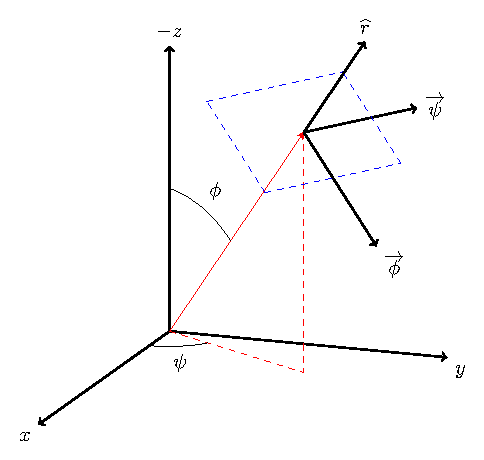
\includepdf{./illustration/repereSiCP.pdf}

\begin{center}
	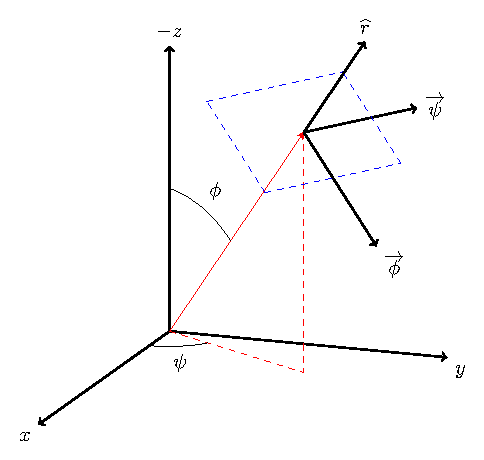
\includegraphics[scale=.97]{./illustration/repereSiCP}
\end{center}

	$\overrightarrow{r}  = \text{} .
	\begin{pmatrix}
		\cos \psi . \sin \phi \\
		\sin \psi . \sin \phi \\
		\cos \phi
	\end{pmatrix}$,

	$\overrightarrow{\psi} = \text{largeur} .
	\begin{pmatrix}
		- \sin \psi \\
		\cos \psi \\
		0
	\end{pmatrix}$,

	$\overrightarrow{\phi} = \text{hauteur} .
	\begin{pmatrix}
		- \cos \psi . \cos \phi \\
		- \sin \psi . \cos \phi \\
		\sin \phi
	\end{pmatrix}$.
%
\subsection{Mathématique}
\begin{description}[leftmargin=0.1cm, itemsep=5pt]
\item{\bf System} : $\theta _\text{i}$.
\item{\bf Chaine} : {\bf r}$_\text{i}$.
\item{\bf Support} : {\bf R}$_\text{i}$.
\item{\bf Point de vue} : {\bf M}, {\bf i}$_\text{M}$,
                                   {\bf j}$_\text{M}$,
                                   {\bf k}$_\text{M}$.
\end{description}
\subsection{Classes}
\begin{description}[leftmargin=0.1cm, itemsep=5pt]
\item{\bf System} : nouveau[N].
\item{\bf Chaine} : chaine[N], support[12], largeur, hauteur.
\item{\bf Point de vue} : perspective, distance, psi, phi.
\end{description}
\subsection{Projection}
\begin{description}[leftmargin=0.1cm, itemsep=5pt]
\item{\bf System-Chaine} : r$_\text{i} = 
	\begin{pmatrix}
		\text{largeur} / 2 \text{N} ( \text{i} - \text{N} / 2 ) \\
		\text{hauteur}. \sin \theta _\text{i} \\
		\text{hauteur}. \cos \theta _\text{i}
	\end{pmatrix}$.
\item{\bf Point de vue} : 
	$\overrightarrow{r}  = \text{} .
	\begin{pmatrix}
		\cos \psi . \sin \phi \\
		\sin \psi . \sin \phi \\
		\cos \phi
	\end{pmatrix}$,
	$\overrightarrow{\psi} = \text{largeur} .
	\begin{pmatrix}
		- \sin \psi \\
		\cos \psi \\
		0
	\end{pmatrix}$,
	$\overrightarrow{\phi} = \text{hauteur} .
	\begin{pmatrix}
		- \cos \psi . \cos \phi \\
		- \sin \psi . \cos \phi \\
		\sin \phi
	\end{pmatrix}$.
\item{\bf Chaine-Rendu} : $\text{g}_\text{i} = 
	\begin{pmatrix}
	(\text{\bf r}_\text{i} - \text{\bf M}).{\text{\bf k}}_\text{M} + \text{hauteur} / 2 \\
	(\text{\bf r}_\text{i} - \text{\bf M}).{\text{\bf j}}_\text{M} + \text{largeur} / 2
	\end{pmatrix}$.
\end{description}
%%%%%%%%%%%%%%%%%%%%%%%%%%%%%%%%%%%%%%%%%%%%%%%%%%%%%%%%%%%%%%%%%%%%%%%%%%%%%%%%%%%%%

%
%%%%%%%%%%%%%%%%%%%%%%%%%%%%%%%%%%%%%%%%%%%%%%%%%%%%%%%%%%%%%%%%%%%%%%%%%%%%%%%%%%%%

%
\chapter{Développement}

Ce chapitre traite de la structure et du développement des programmes de simulation.

%
%%%%%%%%%%%%%%%%%%%%%
\section{Langage et librairies}
%%%%%%%%%%%%%%%%%%%%%
%
%
\subsection{C et SDL2}
%
SiCP2 écrit en C \cite{guide-C} \cite{langage-C} et utilise la librairie SDL2. L'utilisation de la librairie SDL permet la réalisation de l'interface graphique et dynamique avec l'utilisateur.
%
%
%%%%%%%%%%%%%%%%%%%%%%%%%%%%%%%%%%%%%%%%%%%%%%%%%%%%%%%%%%%%%%%%%%%

%
%%%%%%%%%%%%%%%%%%%%%
\section{Modèle Vue Controleur}
%%%%%%%%%%%%%%%%%%%%%
%
%
\subsection{Les répertoires du code source}
\begin{itemize}[leftmargin=2cm]
\item \texttt{donnees} : Inclusion des librairies, constantes et valeurs initiales du système et du graphisme
\item \texttt{fonctions} : Outils mathématique. Fonctions et projection du système
\item \texttt{modele} : Système simulé. 
\item \texttt{graphisme} : Représentation graphique et affichage
\item \texttt{controle} : Liaison entre le système et l'interface graphique 
\item \texttt{objet} : Répertoire pour la compilation
\end{itemize}
%
\subsection{Le modèle}
Le système est un ensemble de pendules couplés
%
\subsection{La vue}
Construit une représentation graphique du système et affiche celle-ci.
%
\subsection{Le controleur}
Exécute alternativement la vue et le modèle. Exécute les actions du clavier.
%
%%%%%%%%%%%%%%%%%%%%%%%%%%%%%%%%%%%%%%%%%%%%%%%%%%%%%%%%%%%%%%%%%%%

%
%%%%%%%%%%%%%%%%%%%%%
\section{Diagrammes}
%%%%%%%%%%%%%%%%%%%%%
%
%\subsection{Cas d'utilisation}
%
\subsection{Inclusion des fichiers dans SiCP2}
%
\begin{center}
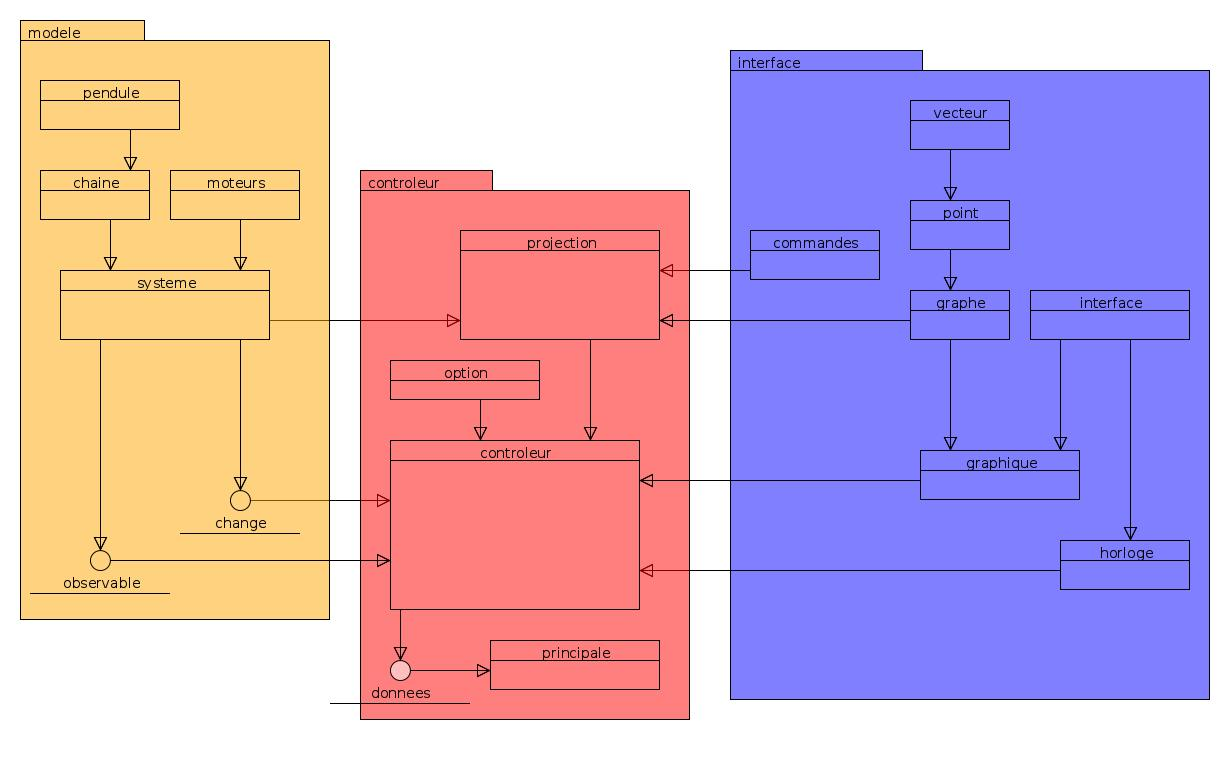
\includegraphics[scale=0.361]{./illustration/diagramme/inclusionsSiCP2}
\end{center}
%
\subsection{diagramme de classes de SiCP2}
\begin{center}
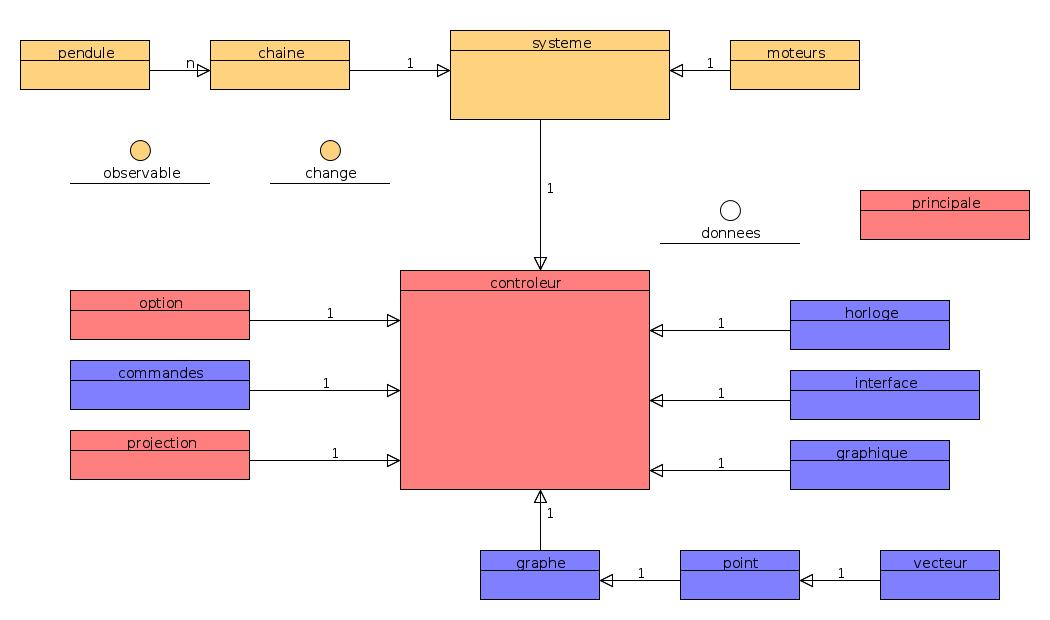
\includegraphics[scale=0.461]{./illustration/diagramme/classesSiCP2}
\end{center}
%
%%%%%%%%%%%%%%%%%%%%%%%%%%%%%%%%%%%%%%%%%%%%
%%%%%%%%%%%%%%%%%%%%%%%%%%%%%%%%%%%%%%%%%%%%
%\begin{itemize}[leftmargin=2cm]
%\item \texttt{gras} : texte
%\end{itemize}



%%%%%%%%%%%%%%%%%%%%%%%%%%%%%%%%%%%%%%%%%%%%%%%%%%%%%%%%%%%%%%%%%%%%%%%%%%%%%%%%%%%%%

%%
%%%%%%%%%%%%%%%%%%%%%
\section{Evolution}
%%%%%%%%%%%%%%%%%%%%%
%
%
\subsection{La branche ted}
Acronyme de "toujours en dévelopement" la version ted des simulateurs teste les dernieres évolutions.
%
\subsection{Sensibilité aux conditions initiales}
Le controleur actuel des simulateurs possède un unique système. Un second système devrait lui être attribué afin d'observer simultanément l'évolution de deux systèmes et d'observer ainsi la sensibilité aux conditions initiales.
%
\subsection{Enregistrement des situations}
La classe fichier enregistre la situation et permet l'initialisation du système. Fonctionelle dans SiCP, elle doit être intégrée dans la version 2 des simulateur.
L'enregistrement et le chargement des positions sont fonctionnels dans SiCF2.
%
%\subsection{}
%
%
%%%%%%%%%%%%%%%%%%%%%%%%%%%%%%%%%%%%%%%%%%%%%%%%%%%%%%%%%%%%%%%%%%%

%%
%%%%%%%%%%%%%%%%%%%%%
\section{Valeurs implicites}
%%%%%%%%%%%%%%%%%%%%%
%
%
\subsection{Réglage de dt, durée et pause}
Une incrémentation du système correspond à une avancée dans le temps de \texttt{dt}. La longueur des pendules est fixé à 25 cm afin de battre la seconde :
Période égale à une seconde
\begin{center}
	\begin{tabular}{rcccl}
	T & = & 2$\pi \sqrt{l/g}$ & = & 1\\
	g/l & = & 4$\pi^2$ & = & 39,478\\
	l & = & 0,25 cm &\\
	\end{tabular}
\end{center}
Empiriquement, un affichage graphique par 30 ms, est obtenue avec une pause de l'ordre de 25ms. Si à chaque affichage correspond à une centaine d'incrémentation de dt, 
\begin{center}
	\begin{tabular}{rcl}
	dt $\times$ duree & = & delay\\
	dt $\times$ 100 & = & 0,03\\
	dt & = & 0,0003\\
	\end{tabular}
\end{center}
La valeur de\texttt {duree} peut être changée dynamiquement avec les touches \texttt{F11} et \texttt{F12} afin de faire varier la vitese de la simulation. La valeur de dt peut être réglée avec l'option \texttt{dt} au démarrage du programme, celle de delay par l'option \texttt{pause}.
Dans SiCP, les valeurs implicites de \texttt{dt} et \texttt{duree} sont égale à 0,0003 et 91, celle de pause est égale à 25. Ces valeurs peuvent être affinée suivant le microprcesseur afin d'avoir un pendule qui bat la seconde.
%
%
\subsection{Limite infinie}
La touche \texttt{v} supprime les frottements sauf pour les derniers pour lesquels les frottements s'accroissent. Ceci permet d'obtenir une extrémité "absorbante".
\begin{itemize}[label=\ding{32}, leftmargin=2cm]
\item pendule de  « précédent »  à  «  nombre $\times$ 5 / 6 » : dissipation de 10 à 1,
\item pendule précédents : dissipation = 0,0
\end{itemize}
%
%
\subsection{dt et dissipation maximale}
La touche \texttt{v} supprime les frottements sauf pour les derniers pour lesquels les frottements s'accroissent. Ceci permet d'obtenir une extrémité "absorbante".
\begin{center}
	\begin{tabular}{rcl}
	dt $\times$ DISSIPATION\_MAX & = & constante\\
	0.0003 $\times$ 333 & = & 0,0999\\
	dissipation maximale & = & 0,0999/dt\\
	\end{tabular}
\end{center}
%
%
\subsection{Limitation des valeurs des variables}
%
\subsubsection{Paramètres physiques}
%
Au delà de certaines valeurs de certain paramètres dynamiques, la simulation s'éloigne du comportement physique.
%
\begin{itemize}[label=\ding{32}, leftmargin=2cm]
\item Pour des raisons de discrétisation
\item En raisons de possibles erreurs d'algorithme
\item En raisons de possibles erreurs d'écriture
\end{itemize}
%
Aussi, le fichier \texttt{donnees/constantes.c} contient des valeurs maximale et minimale de certains paramètres. Ces bornes permettent de consolider le comportement des programmes.

En particulier, dans le calcul de la représentation du graphe de SiCP, les coordonées polaires du point de vue sont bornées, $\phi$ ne peut pas être égale à zéro, sa valeur minimale est égale à \texttt{EPSILON} afin d'éviter un plantage due à l'algorithme simplifiée de la représentation graphique.
%
\subsubsection{Paramètres dynamiques}
%
\begin{itemize}[label=\ding{32}, leftmargin=2cm]
\item Vitesse des mobiles
\item Distance entre les mobiles
\item Énergie
\end{itemize}
%
Actuellement, l'angle des pendules de SiCP est borné grâce à une fonction de jauge ramenant la position du premier pendule entre -$\pi$ et $\pi$.
Un test sur la valeur de l'énergie et la limitation de celle-ci permetrait sans doute de consolider davantage le programme. En effet, parmi les bug connus, une valeur trop grande des variables apparait en premier lieu dans la valeur de l'énergie totale.

Ainsi, afin de limiter la vitesse des mobiles, la position des mobiles pourrait être divisées par deux dans les équations linéaires lorsque l'énergie totale est supérieur à \texttt{ENERGIE\_SECURITE}.
%\subsubsection{Énergie maximale}
%La valeur de l'énergie permetrait de limiter un certain nombres d'erreurs.
%
%Lorsque l'énergie est supérieur à ENERGIE\_SECURITE, La position des mobiles pourrait être divisées par deux dans les équations linéaires
%\begin{center}
%	\begin{tabular}{rcl}
% &  &1 009 200 790 976 791 136 174 080\\
% &  &  585 891 747 701 731 153 149 952\\
%      999000555444333222111\\
%\multicolumn{3}{c}{\#define ENERGIE\_SECURITE 777666555444333222111}\\
%	\end{tabular}
%\end{center}
%

%%%%%%%%%%%%%%%%%%%%%%%%%%%%%%%%%%%%%%%%%%%%%%%%%%%%%%%%%%%%%%%%%

%
%
%
\begin{appendix}
%%%%%%%%%%%%%%%%%%%%%%%%%%%%%%%%%%
\chapter{Première version des simulateurs}
%%%%%%%%%%%%%%%%%%%%%%%%%%%%%%%%%%

%\chapter{Présentation et installation}
%%%%%%%%%%%%%%%%%%%%%%%%%%%%%%%%%%
%
%%%%%%%%%%%%%%%%%%%%%%%%%%%%%%%%%%

\section{Historique}
%
La première version des simulateurs utilisait la librairie SDL 1.2. Cette librairie a évolué vers la version SDL2. Les programmes décrit dans cette documentation ont donc évolué vers une version 2 utilisant la nouvelle librairie. Les versions 1.x des simulateurs sont donc vouées à ne plus être maintenues. Aujourd'hui, les versions 2 des simulateurs disposent d'une interface graphiques plus conviviale avec une interaction avec la souris. La commande des simulateurs à l'aide du clavier reste fonctionelle et est décrite dans l'annexe suivante.
%%%%%%%%%%%%%%%%%%%%%%%%%%%%%%%%%%%%%%%%%%%%%%%%%%%%%%%%%%%%%%%%%%%%%%%%%%%%%%%%%%%%%%%%%%%%%

\newpage
%%%%%%%%%%%%%%%%%%%%%%%%%%%%%%%%%%
\chapter{Commandes du clavier}
%%%%%%%%%%%%%%%%%%%%%%%%%%%%%%%%%%

%
\section{Résumé du clavier SiCF et SiCP}
%
Le clavier permet de modifier les paramètres physiques. La fenêtre graphique doit être active, le terminal affiche les informations.
%
%
% V1
%Le clavier permet de modifier les paramètres physiques. La fenêtre graphique doit être active, le terminal affiche les informations.
\footnotesize
\begin{center}
\begin{tabular}{cccccccccc}
%\sffamily
%\rmfamily
\sf A &\sf Z &\sf E &\sf R &\sf T &\sf Y &\sf U &\sf I &\sf O &\sf P \\
Couplage & Masse & Dissip. & supprimD & Gravit. & Phi & Ampl. & impuls. & sinus & Fréquence \\
\sf Q &\sf S &\sf D &\sf F &\sf G &\sf H &\sf J &\sf K &\sf L &\sf M \\
moinsC & moinsM & plusD & formeD & moinsG & moins$\Phi$ & moinsA &  & carré & moinsF \\
\sf W &\sf X &\sf C &\sf V &\sf B &\sf N &  &  &  & \\
périodique & libres & fixe & ExtAbsD & libFix & fixLib &  &  &  & \\
\end{tabular}
\end{center}
\vspace{.3cm}
%
\normalsize
\begin{itemize}[leftmargin=2cm, label=\ding{32}, itemsep=0pt]%\end{itemize}
\item Paramètres physiques

\begin{tabular}{ccccc}
%\sffamily
%\rmfamily
\sf A &\sf Z &\sf E &\sf R &\sf T  \\
Couplage & Masse & Dissip. & supprimD & Gravit.  \\
\sf Q &\sf S &\sf D &\sf F &\sf G  \\
moinsC & moinsM & plusD & formeD & moinsG  \\
 & & & \sf V   & \\
 & & & ExtAbsD &  \\
\end{tabular}
%
\end{itemize}
\begin{itemize}[leftmargin=2cm, label=\ding{32}, itemsep=0pt]%\end{itemize}
\item Conditions aux limites

\hspace{3cm}
\begin{tabular}{cccccccccc}
%\sffamily
%\rmfamily
 & & & &\sf Y \\
 & & & & Phi \\
 & & & &\sf H \\
 & & & & moins$\Phi$  & & &  & \\
\sf W &\sf X &\sf C &\sf V &\sf B &\sf N  \\
périodique & libres & fixe &  & libFix & fixLib  \\
\end{tabular}
%
\end{itemize}
\begin{itemize}[leftmargin=2cm, label=\ding{32}, itemsep=0pt]%\end{itemize}
\item Moteur premier pendule

\hspace{9cm}
\begin{tabular}{ccccc}
%\sffamily
%\rmfamily
\sf U &\sf I &\sf O &\sf P \\
 Ampl. & impuls. & sinus & Fréquence \\
\sf J &\sf K &\sf L &\sf M \\
 moinsA &  & carré & moinsF \\
\end{tabular}
%
\end{itemize}
%\vspace{.3cm}
Les touches de fonctions donnent un certain nombre de contrôles et d'information:
%
\begin{center}
\begin{tabular}{ccccc ccccc cc}
\multicolumn{4}{|c|}{Contrôles} & \multicolumn{4}{c}{Information} & \multicolumn{4}{|c|}{Contrôles}\\
\sf F1 &\sf F2 &\sf F3 &\sf F4 &\sf F5 &\sf F6 &\sf F7 &\sf F8 &\sf F9 &\sf F10 &\sf F11 &\sf F12 \\
\multicolumn{4}{|c|}{Équation simulé (SiCF)} & \multicolumn{4}{c}{Énergie, graphe} & \multicolumn{4}{|c|}{Vitesse de la simulation}\\
\end{tabular}
\end{center}
%
Le choix de l'équation simulée est spécifique à SiCF. {\sf F5} dresse un bilan énergétique. {\sf F6} affiche les paramètres physiques du système
\begin{center}
\begin{tabular}{cccccc}
\sf F1 &\sf F2 &\sf F3 &\sf F4 &\sf F5 &\sf F6\\
Pendules & Harmoniques & Corde & asymétrique & Énergie & Système \\
\end{tabular}
\end{center}
%
{\sf F8} permet de modifier  le graphisme de SiCP. {\sf F9} et {\sf F12} modifient rapidement le rythme de la simulation, {\sf F10} et {\sf F11} la modifie modéremment. La touche {\sf Entrée} change le mode avec ou sans attente, en mode avec attente, l'appuie sur une touche permet l'évolution du système.
\begin{center}
\begin{tabular}{cccccc}
\sf F8 &\sf F9 &\sf F10 &\sf F11 &\sf F12 & \sf Entrée \\
Support (SiCP) & -Sim & -Sim & +Sim & +Sim & mode\\
\end{tabular}
\end{center}
%
\section{Détails des contrôles}
%
%\begin{itemize}[leftmargin=1cm, label=\ding{32}, itemsep=0pt]
%
\subsection{Équation simulée}
%
Il s'agit d'une spécificité de SiCF. Lorsque le mode asymétrique est activé, les touches {\sf z} et {\sf s} ne change la masse de la corde que pour la moitié droite. 
%
\begin{itemize}[leftmargin=2cm, label=\ding{32}, itemsep=0pt]%\end{itemize}
\item 1: {\bf gravitation} forceRappel = sinus de la position du pendule
\item 2: {\bf linearisation} forceRappel = proportionnelle à la position du pendule
\item 3: {\bf corde vibrante} forceRappel = 0
\item 4: {\bf corde vibrante asymétrique} permet de changer la masse sur une demi-corde.
\end{itemize}
%
\subsection{Paramètres des pendules}
%
\begin{itemize}[label=\ding{32}, leftmargin=2cm, itemsep=0pt]
\item {\bf Couplage} : {\sf a}, {\sf q} : Augmente, diminue le couplage entre les pendules.
\item {\bf Masse} : {\sf z}, {\sf s} :  Augmente, diminue la masse des pendules.
\item {\bf Dissipation} : {\sf e}, {\sf d} :  Augmente, diminue les frottements visqueux.
\item {\bf Gravitation} : {\sf t}, {\sf g} :  Augmente, diminue l'accélération de la gravitation.
%\item {\bf } : \sf{} : 
\end{itemize}
%
%
\subsection{Forme de la dissipation}
%
La touche {\sf V} supprime les frottements sauf pour les derniers pour lesquels les frottements s'accroissent. Ceci permet d'obtenir une extrémité "absorbante", permettant la simulation d'une corde infinie.
%
\begin{itemize}[label=\ding{32}, leftmargin=2cm, itemsep=0pt]
\item {\bf Supprimer} : {\sf e} : Supprime les frottements visqueux.
\item {\bf Former} : {\sf f} : Active les frottements visqueux sur toute la chaîne.
\item {\bf Absorber} : {\sf v} : Active les frottements visqueux sur la fin de la chaîne, crée une extrémité absorbante.
\end{itemize}
%
%
\subsection{Conditions aux limites}
%
\begin{itemize}[label=\ding{32}, leftmargin=2cm, itemsep=0pt]
\item {\bf Périodique} : {\sf w} : Le dernier pendule est couplé au premier.
\item {\bf Libres} : {\sf x} : Les deux extrémités sont libres.
\item {\bf Fixes} : {\sf c} : Les deux extrémités sont fixes.
\item {\bf libre-fixe} : {\sf b} : Le premier pendule est libre et le dernier pendule est fixe.
\item {\bf fixe-libre} : {\sf n} : Le premier pendule est fixe et le dernier pendule est libre.
\end{itemize}
%
%
\subsection{Moteur premier pendule}
%
\begin{itemize}[label=\ding{32}, leftmargin=2cm, itemsep=0pt]
\item {\bf Impulsion} : {\sf i} : Crée une impulsion.
\item {\bf Sinus} : {\sf o} : Active, désactive le moteur sinusoïdale.
\item {\bf Sinus} : {\sf l} : Active le moteur carré.
\item {\bf Amplitude} : {\sf u, j} :  Augmente, diminue l'amplitude du moteur.
\item {\bf Fréquence} : {\sf p, m} :  Augmente, diminue la fréquence du moteur.
\end{itemize}
%
%
\subsection{Moteur Josephson}
%
\begin{itemize}[label=\ding{32}, leftmargin=2cm, itemsep=0pt]
\item {\bf Activation} : $\rightarrow$ : Crée, supprime un courant josephson.
\item {\bf Amplitude} : $\mathtt{\uparrow}$, $\mathsf{\downarrow}$ : Augmente, diminue le courant.
\item {\bf Sens} : {\sf $\leftarrow$} : Inverse le sens du courant josephson.
%\item {\bf } : \sf{} : 
\end{itemize}
%
%
\subsection{Contrôle de la simulation}
%
{\sf F9} et {\sf F12} modifient rapidement la vitesse de la simulation, {\sf F10} et {\sf F11} la modifient modéremment. La touche {\sf Entrée} change le mode avec ou sans attente, en mode avec attente, l'appuie sur une touche permet l'évolution du système.
%
\begin{itemize}[label=\ding{32}, leftmargin=2cm, itemsep=0pt]
\item {\bf Mode} : {\sf Entrée} : Change le mode de la simulation : évolution automatique ou pas à pas.
\item {\bf Accélèrer} : {\sf 11} et {\sf F12} : Accélère la simulation.
\item {\bf Ralentir} : {\sf F9} et {\sf F10} : Ralentit la simulation.
\end{itemize}
%
%
\subsection{Information}
\begin{itemize}[label=\ding{32}, leftmargin=2cm, itemsep=0pt]
\item {\bf Énergie} : {\sf F5} : Information énergétique de la chaîne.
\item {\bf Système} : {\sf F6} : Affiche les paramètres physiques du système.
%\item {\bf } : \sf{F7} : 
%\item {\bf } : \sf{F8} : 
\end{itemize}
%
\subsection{Sauvegarde et ré-initialisation dans SiCF}
%
Cette fonctionnalité nécessite la présence du répertoire {\texttt donnee/enregistrement} dans le répertoire de l'exécutable.
La touche majuscule permet d'accéder aux fonctions d'enregistrement et de ré-initialisation des positions des pendules.

Lorsque la touche majuscule est enfoncé, les touches {\sf A}, {\sf Z}, {\sf E}, {\sf R}, {\sf T}, {\sf Y}, {\sf U}, {\sf I}, {\sf O} et {\sf P}, ainsi que les touches {\sf J}, {\sf K}, {\sf L} et {\sf M} ré-initialisent la position de la corde dans différentes configurations préréglées.

Les touches {\sf W}, {\sf X}, {\sf C}, {\sf V}, {\sf B} et {\sf N} enregistrent la position de la corde dans l'état actuel, les touches {\sf Q}, {\sf S}, {\sf D}, {\sf F}, {\sf G} et {\sf H} réinitialisent la position de la corde dans ces états enregistés.
%
\subsubsection{Fonction élémentaire}
%
\begin{center}
\begin{tabular}{cc cc}%\multicolumn{4}{|c|}{}\\
Touche & fonction \\
A & nulle &\\
Z & impulsion &\\
E & triangle&\\
R & triangle&\\
T & carré &\\
Y & carré &\\
\end{tabular}
\end{center}
%
\subsubsection{Quanton}
%
\begin{center}
\begin{tabular}{cc cc}%\multicolumn{4}{|c|}{}\\
Touche & fonction \\
U, J & impulsion &\\
I, K & impulsion &\\
O, L & quanton &\\
P, M & quanton &\\
\end{tabular}
\end{center}

\subsubsection{Fichiers de ré-initialisation}
Les fichiers de ré-initialisation se trouvent dans le répertoire {\texttt donnee/enregistrement}. Ils peuvent être édités. Le nom de ces fichiers doit être respecté afin de pouvoir être ouvert par le programme (ces noms sont utilisés par {\texttt donnees/fichier.c}).
%
%\end{itemize}
%
%\item {\bf } : \sf{} : 
%%%%%%%%%%%%%%%%%%%%%%%%%%%%%%%%%%%%%%%%%%%%%%%%%%%%%%%%%
%
%%%%%%%%%%%%%%%%%%%%%%%%%%%%%%%%%%%%%%%%%%%%%%%%%%%%%%%%%%%%%%%%%%%%%%%%%%%%%%%%%%%%%%%%%%%%%

\newpage
%%%%%%%%%%%%%%%%%%%%%%%%%%%%%%%%%%
\chapter{Commandes du clavier}
%%%%%%%%%%%%%%%%%%%%%%%%%%%%%%%%%%

%%%%%%%%%%%%%%%%%%%%%%%%%%%%%%%%%%%%%%%%%%%%%%%%%%%%%%%%%%
%
\section{SiCF et SiCP}
%
%%%%%%%%%%%%%%%%%%%%%%%%%%%%%%%%%%%%%%%%%%%%%%%%%%%%%%%%%%
%
Lorsque le programme est démarré en ligne de commande, il est possible de passer un certain nombre d'options. Ces options sont communiquées au programme à l'aide du nom de l'option suivie d'un nombre. Par exemple pour démarrer SiCF avec un fond sombre et une discrétisation du temps égale à 0,00033 seconde :
\begin{center}
\texttt{./SiCF fond 17 dt 0.00033}
\end{center}
Pour démarrer SiCP avec un fond sombre, un nombre de pendules égale à 50 et trois solitons :
\begin{center}
\texttt{./SiCP fond 17 soliton 3 nombre 50}
\end{center}
%
Pour démarrer SiCP en exploitant plusieurs options :
\begin{center}
\texttt{./SiCP fond 45 support 0 pause 7 duree 998 dt 0.0027 nombre 777 soliton 18}
\end{center}
%
\subsection{Résumé des options}
\begin{center}
\begin{tabular}{cccc}
option & valeur & clavier & commande \\
%\hline
{\texttt fond} & (fond>0 \& fond<255) &  & Couleur du fond ***\\
{\texttt soliton} & (soliton > -99 \& soliton < 99) & {\sf y},{\sf h} & déphasage entre les extrémitées *\\
{\texttt dt} & (dt > 0.0 \& dt < DT\_MAX) &  & discrétisation du temps \\
{\texttt frequence} & () & {\sf p}, {\sf m} & fréquence du générateur \\
{\texttt dissipation} & () & {\sf e}, {\sf d} & dissipation \\
{\texttt equation} & (equation > 0 \& equation < 5) & {\sf F1}, {\sf F2}, {\sf F3}, {\sf F4} & choix de l'équation \\
{\texttt pause} & (pause > 5 || pause < 555) &  & temps de pause en ms \\
{\texttt duree} & () & {\sf F9}, {\sf F10}, {\sf F11}, {\sf F12} & rythme de la simulation \\
{\texttt mode} & () & {\sf Entrée} & Mode -1 : Wait, 1 : Poll \\
{\texttt nombre} & (nombre > 0 \& nombre < 1099) &  & Nombre de pendules **\\
{\texttt aide} & () &  & Affiche l'aide \\
{\texttt help} & () &  & Affiche l'aide \\
\end{tabular}
\end{center}

{\it
* Initialise le déphasage entre le dernier pendule et le premier pendule dans le cas des conditions aux limites périodique.

** Spécifique à SiCP, nombre < 399 dans SiCP2.

*** Désactivé dans les versions 2.
}
%

%
\end{appendix}
%

%
%
%====================== INCLUSION DE LA BIBLIOGRAPHIE ======================
%
%récupérer les citation avec "/footnotemark"
%\nocite{*}
%choix du style de la biblio
\bibliographystyle{plain}
%inclusion de la biblio
\cleardoublepage
\addcontentsline{toc}{chapter}{Bibliographie}
\bibliography{bibliographie.bib}
%\newpage
%\input{./glossaire/glossaire.tex}
%\newpage
%\input{./annexes/annexes.tex}
\end{document}
%%%%%%%%%%%%%%%%%%%%%%%%%%%%%%%%%%%%%%%%%%%%%%%%%%%%%%%%%%%%%%%%%%%%%%%%%%%%%%%%%
